%!TeX root=./ordenacao.tex


\section{Árvore binária balanceada de busca} \label{sec:abb}

Manter um vetor ordenado é uma boa maneira de resolver o problema da
lista ordenada cinética dando suporte às operações
\textsc{advance}$(t)$, \textsc{change}$(j,v)$ e
\textsc{query\_kth}$(i)$.
Poderíamos também querer dar suporte, além das operações citadas, às seguintes operações:

\begin{itemize}
    \item \textsc{insert}$(v, x_t) \rightarrow$ insere um
    elemento com velocidade $v$ e valor $x_t$ no instante \now;
    \item \textsc{delete}$(i) \rightarrow$ remove o elemento
    $i$ no instante \now.
\end{itemize}

Para inserir um elemento no vetor ordenado, antes teríamos de
encontrar a posição $j$ que o elemento deveria ocupar no vetor.
Movemos todos os elementos, a partir da posição $j$, uma posição à
frente e colocamos o elemento novo na posição~$j$.
Simultaneamente movemos os certificados correspondentes uma posição para frente, criamos um novo
certificado entre o novo elemento e seu predecessor e também atualizamos o certificado do seu
sucessor.
As alterações correspondentes também devem ser feitas na fila $Q$ e nos vetores $\textit{indS}$ e
$\textit{indQ}$.
%Após isso, os certificados de $j$~até~$n-1$ devem ser atualizados, pois esses elementos mudaram de
%posição no vetor, e um novo certificado será criado, o $n$-ésimo
%certificado.
%Ademais, o total de elementos $n$ deve ser mudado para $n + 1$.
%O novo certificado também deve ser inserido na fila com prioridades.

Só a operação de inserir um novo elemento no vetor já pode se tornar
pouco eficiente com uma grande quantidade de elementos sendo
inseridos no começo do vetor, consumindo tempo linear por inserção.
Como a remoção de um elemento no vetor ordenado envolve uma
sequência parecida de operações, da mesma maneira se torna pouco
eficiente, também consumindo tempo linear no pior caso.

Dessa forma, apesar da lista ordenada cinética implementada
manipulando um vetor ser uma estrutura eficiente para a operação
\textsc{query\_kth}$(i)$, com um consumo de tempo constante, o
consumo de tempo para as operações \textsc{insert}$(v, x_t)$ e
\textsc{delete}$(i)$ é, no pior caso, proporcional ao número de
elementos, o que pode ser ruim para uma grande quantidade de
elementos, inserções e remoções.

Podemos equilibrar o consumo de tempo das operações
\textsc{query\_kth}$(i)$, \textsc{insert}$(v, x_t)$ e
\textsc{delete}$(i)$ em tempo logarítmico no número de elementos,
usando uma árvore binária balanceada de busca (ABBB) em vez do vetor $\sorted$.
Os pontos serão armazenados na ABBB tendo o seu valor no instante \now~como
chave.

Além da ABBB, para garantirmos a eficiência das operações
\textsc{event}, \textsc{change}, \textsc{insert} e \textsc{delete},
cada elemento terá um apontador para o seu predecessor na ABBB e um
apontador para o seu sucessor, formando uma lista duplamente ligada
ordenada pelo valor do elemento no instante \now; veja a Figura~\ref{fig:abb:exemplo}.

\begin{figure}[H]
    \centering
    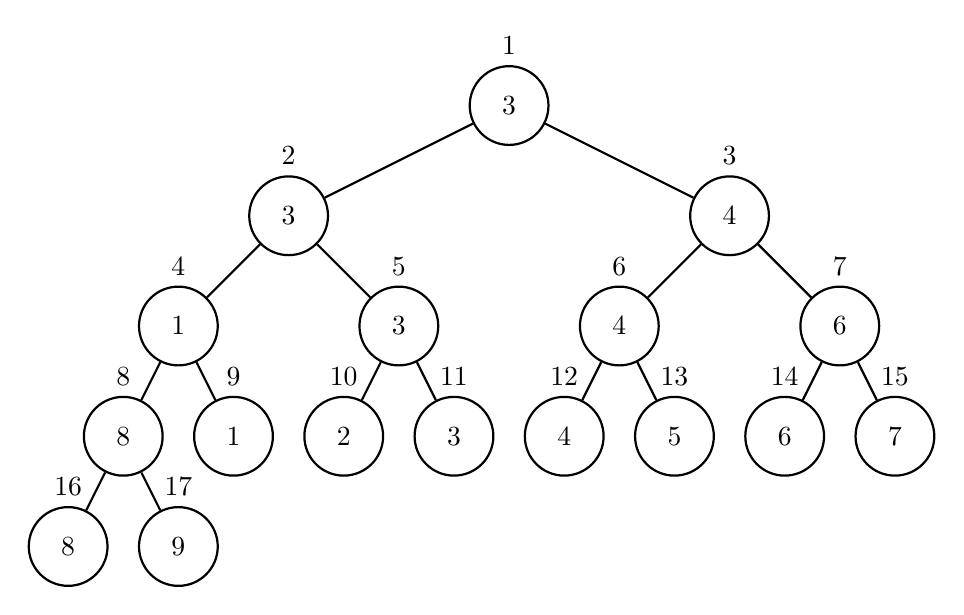
\begin{tikzpicture}[thick, scale=0.7]
        \node[label={1},circle,draw,minimum size=1cm]
        (1) at (0,0) {$3$};
        \node[label={2},circle,draw,minimum size=1cm]
        (2) at (-4,-2) {$3$};
        \node[label={3},circle,draw,minimum size=1cm]
        (3) at (4,-2) {$4$};
        \node[label={4},circle,draw,minimum size=1cm]
        (4) at (-6,-4) {$1$};
        \node[label={5},circle,draw,minimum size=1cm]
        (5) at (-2,-4) {$3$};
        \node[label={6},circle,draw,minimum size=1cm]
        (6) at (2,-4) {$4$};
        \node[label={7},circle,draw,minimum size=1cm]
        (7) at (6,-4) {$6$};
        \node[label={8},circle,draw,minimum size=1cm]
        (8) at (-7,-6) {$8$};
        \node[label={9},circle,draw,minimum size=1cm]
        (9) at (-5,-6) {$1$};
        \node[label={10},circle,draw,minimum size=1cm]
        (10) at (-3,-6) {$2$};
        \node[label={11},circle,draw,minimum size=1cm]
        (11) at (-1,-6) {$3$};
        \node[label={12},circle,draw,minimum size=1cm]
        (12) at (1,-6) {$4$};
        \node[label={13},circle,draw,minimum size=1cm]
        (13) at (3,-6) {$5$};
        \node[label={14},circle,draw,minimum size=1cm]
        (14) at (5,-6) {$6$};
        \node[label={15},circle,draw,minimum size=1cm]
        (15) at (7,-6) {$7$};
        \node[label={16},circle,draw,minimum size=1cm]
        (16) at (-8,-8) {$8$};
        \node[label={17},circle,draw,minimum size=1cm]
        (17) at (-6,-8) {$9$};

        \draw[thick] (1) -- (2);
        \draw[thick] (2) -- (4);
        \draw[thick] (4) -- (8);
        \draw[thick] (4) -- (9);
        \draw[thick] (8) -- (16);
        \draw[thick] (8) -- (17);
        \draw[thick] (2) -- (5);
        \draw[thick] (5) -- (10);
        \draw[thick] (5) -- (11);
        \draw[thick] (1) -- (3);
        \draw[thick] (3) -- (6);
        \draw[thick] (3) -- (7);
        \draw[thick] (6) -- (12);
        \draw[thick] (6) -- (13);
        \draw[thick] (7) -- (14);
        \draw[thick] (7) -- (15);
    \end{tikzpicture}
    \caption[Representação da estrutura torneio]{Torneio com $9$
        elementos em que $3$ é o elemento com valor máximo.}
    \label{fig:torneio:exemplo}
\end{figure}

No que diz respeito aos certificados, antes um certificado estava
associado a uma posição e, no vetor, ao inserirmos um elemento em
uma determinada posição, teríamos que deslocar % que atualizar
todos os certificados conseguintes àquela posição.
Agora, para que consigamos alterar apenas uma quantidade constante de certificados
após uma inserção, os certificados não estarão mais associados a uma
posição e sim aos elementos.
Ou seja, o certificado $i$ se refere à relação estabelecida entre o elemento $i$ e seu predecessor
e consiste no instante de tempo em que o elemento $i$ deixará de ter um valor maior que o valor do
seu predecessor, se esse instante for maior que o instante atual.
Do contrário, o certificado consiste em $+\infty$.
Se o elemento $i$ não possui predecessor, então o certificado também consiste em
$+\infty$.
Veja a Figura~\ref{fig:abb:cert}.

\begin{figure}[htb]
    \centering
    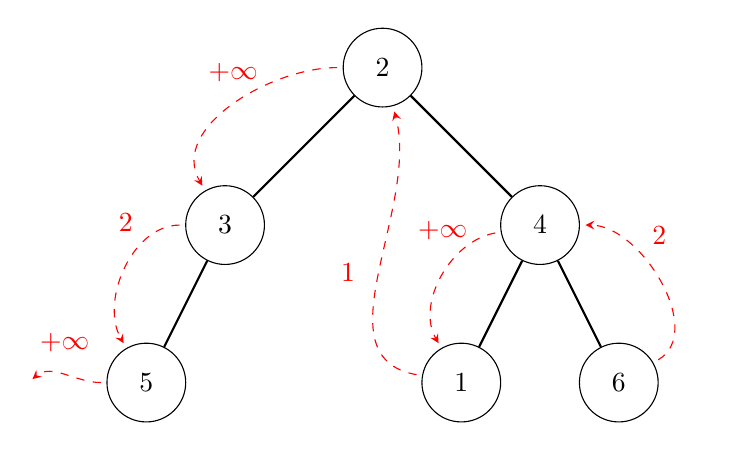
\begin{tikzpicture}[baseline=-2.25cm]
        \node[circle,draw,minimum size=1cm] (1) at (0,0)  {$2$};
        \node[circle,draw,minimum size=1cm] (2) at (-2,-2){$3$};
        \node[circle,draw,minimum size=1cm] (3) at (2,-2) {$4$};
        \node[circle,draw,minimum size=1cm] (4) at (-3,-4){$5$};
        \node[circle,draw,minimum size=1cm] (5) at (1,-4) {$1$};
        \node[circle,draw,minimum size=1cm] (6) at (3,-4) {$6$};
        \tikzstyle{filho}=[thick]
        \tikzstyle{pred}=[->, shorten >= 2pt, shorten <= 2pt,
        dashed, >=stealth, red]
        \tikzstyle{sucessor}=[->, shorten >= 2pt, shorten <= 2pt,
        dotted, >=stealth, line width=0.35mm]
        \draw[filho] (1) -- (2);
        \draw[filho] (1) -- (3);
        \draw[filho] (2) -- (4);
        \draw[filho] (3) -- (5);
        \draw[filho] (3) -- (6);
        \draw[pred] (6) edge[out=30,in=0] node[above=10pt, red] {$2$} (3);
        % \node[red] at (4,-3) {$2$};
        \draw[pred] (3) edge[out=190,in=120]
        node[above=10pt, red] {$+\infty$} (5);
        \draw[pred] (5) edge[out=170,in=285]
        node[left=5pt, red] {$1$} (1);
        \draw[pred] (1) edge[out=180,in=120]
        node[above=5pt, red] {$+\infty$} (2);
        \draw[pred] (2) edge[out=180,in=120]
        node[above=10pt, red] {$2$} (4);
        \draw[pred] (4) edge[out=180,in=40]
        node[above=5pt, red] {$+\infty$} (-4.5, -4);
    \end{tikzpicture}
    \qquad
    \qquad
    \qquad
    \begin{tabular}{|c|c|c|c|}
        \hline
        $i$ & $x_0$ & $v$   & $\cert[i]$ \\
        \hline
        $1$ & $6$   & $2$   & $1$        \\

        $2$ & $3$   & $5$   & $+\infty$  \\

        $3$ & $2$   & $1$   & $2$        \\

        $4$ & $7$   & $4$   & $+\infty$  \\

        $5$ & $-2$  & $3$   & $+\infty$  \\

        $6$ & $14$  & $0.5$ & $2$        \\
        \hline
    \end{tabular}
    \caption[Representação dos certificados da ABB]{Certificados
    representados pelas setas vermelhas tracejadas. O
    elemento $5$ é o último da lista e o seu certificado vale $+\infty$.}
    \label{fig:abb:cert}
\end{figure}

Esses $n$ certificados também serão colocados em uma fila com
prioridades, com o prazo de validade determinando a prioridade.
A fila com prioridades agora também deverá suportar operações
como a inserção e remoção de certificados.

Para descrever as implementações das operações, vamos
estabelecer os nomes dos objetos, variáveis e rotinas
auxiliares utilizados:
\begin{enumerate}
    \item $n$: número de elementos no instante \now;
    \item \no: objeto que compõe a árvore binária balanceada
    de busca, com atributos:
    \begin{enumerate}
        \item \esq$:$ aponta para a raiz da subárvore
        esquerda do nó;
        \item \dir$:$ aponta para a raiz da subárvore
        direita do nó;
        \item \textit{key}$:$ aponta para um elemento;
        \item \children$:$ quantidade de nós que a subárvore
        enraizada neste nó possui.
        Este atributo será importante para a operação \textsc{query\_kth}$(i)$;
    \end{enumerate}
    \item \raiz: nó que é a raiz da árvore binária balanceada de
    busca;
    \item \elemento: objeto com os seguintes atributos:
    \begin{enumerate}
        \item \id: vem de \textit{identifier} e é o atributo
        para identificar o elemento.
        Assim, daqui em diante, usaremos elemento $i$ para nos
        referirmos ao elemento cujo \id~é $i$;
        \item \speed: velocidade do elemento;
        \item \initv: valor que o elemento possuía no
        instante~$t = 0$;
        \item \nex: apontador para o elemento imediatamente
        posterior a este na coleção, no instante \now.
        O elemento imediatamente posterior a $i$ é aquele
        que possui o menor valor dentre a coleção de
        elementos que possuem valor maior que o elemento
        $i$;
        \item \prev: apontador para o elemento imediatamente
        anterior a este na coleção, no instante \now; $\nnull$ se o elemento é o primeiro;
        \item \pqpos: aponta para a posição do certificado associado
        ao elemento na fila com prioridades;
        \item \cert: prazo de validade do certificado entre este elemento e o elemento
        apontado por \prev; se \prev~é $\nnull$ \cert~vale $+\infty$;
        \item \no: apontador para o nó da árvore binária de busca em
        que o elemento se encontra;
    \end{enumerate}
    \item \Q: fila com prioridades que contém os elementos;
    o prazo do certificado entre o elemento e seu predecessor é a prioridade do elemento, e o
    elemento com menor prioridade estará à frente da fila;

    \item \textsc{insertKey}$(\text{\raiz},e)\rightarrow$ insere
    $e$, um elemento, na árvore binária balanceada de busca com raiz
    \raiz~e retorna a, possivelmente nova, raiz da árvore.
    No processo também atualiza a lista ligada de elementos;

    \item \textsc{deleteKey}$(\text{\raiz},e)\rightarrow$ remove
    $e$, um elemento, da árvore binária balanceada de busca com raiz
    \raiz~e retorna a, possivelmente nova, raiz da árvore.
    No processo também atualiza a lista ligada de elementos.

\end{enumerate}
Para a implementação das operações \textsc{change}$(j, v)$ e
\textsc{delete}$(i)$, precisamos de alguma maneira recuperar um
elemento baseado no seu \id.
Para tal, podemos utilizar uma tabela de símbolos, implementada por uma árvore binária balanceada
de busca ou uma tabela de dispersão.
A seguir~estão três operações que nos ajudarão a recuperar os elementos:

\begin{enumerate}
    \item \textsc{getObject}$(i)\rightarrow$ retorna o elemento $i$;
    \item \textsc{insertObject}$(e) \rightarrow$ insere $e$,
    que é um elemento, na tabela de símbolos;
    \item \textsc{deleteObject}$(e) \rightarrow$ remove $e$,
    que é um elemento, da tabela de símbolos.
\end{enumerate}

Para permitir a inserção e remoção de certificados, a interface da
fila com prioridades será reformulada, contando com duas operações
extras:

\begin{enumerate}
    \item \textsc{insertPQ}$(Q, e, t) \rightarrow$ insere $(e, t)$
    na fila com prioridades $Q$, sendo $t$ o prazo de validade do certificado de $e$;
    \item \textsc{deletePQ}$(Q, e) \rightarrow$ remove $e$
    da fila com prioridades $Q$;
    \item \textsc{updatePQ}$(Q,e,t) \rightarrow$ muda o prazo de
    validade do certificado de $e$ para $t$ e atualiza a fila com
    prioridades $Q$;
    \item \textsc{minPQ}$(Q) \rightarrow$ devolve o elemento com o
    certificado de menor prazo de validade da fila com prioridades
    $Q$.
\end{enumerate}

A operação \textsc{updatePQ}$(Q,e,t)$ pode ser implementada de modo
a consumir tempo logarítmico no número de elementos em $Q$ graças ao
atributo \pqpos~dos elementos.

\begin{figure}
    \centering
    \begin{tikzpicture}[thick, scale=0.8]
        \node[label={1},circle,draw,minimum size=1cm]
            (1) at (0,0) {$3$};
        \node[label={2},circle,draw,minimum size=1cm]
            (2) at (-4,-2) {$3$};
        \node[label={3},circle,draw,minimum size=1cm]
            (3) at (4,-2) {$4$};
        \node[label={4},circle,draw,minimum size=1cm]
            (4) at (-6,-4) {$1$};
        \node[label={5},circle,draw,minimum size=1cm]
            (5) at (-2,-4) {$3$};
        \node[label={6},circle,draw,minimum size=1cm]
            (6) at (2,-4) {$4$};
        \node[label={7},circle,draw,minimum size=1cm]
            (7) at (6,-4) {$6$};
        \node[label={8},circle,draw,minimum size=1cm]
            (8) at (-7,-6) {$8$};
        \node[label={9},circle,draw,minimum size=1cm]
            (9) at (-5,-6) {$1$};
        \node[label={10},circle,draw,minimum size=1cm]
            (10) at (-3,-6) {$2$};
        \node[label={11},circle,draw,minimum size=1cm]
            (11) at (-1,-6) {$3$};
        \node[label={12},circle,draw,minimum size=1cm]
            (12) at (1,-6) {$4$};
        \node[label={13},circle,draw,minimum size=1cm]
            (13) at (3,-6) {$5$};
        \node[label={14},circle,draw,minimum size=1cm]
            (14) at (5,-6) {$6$};
        \node[label={15},circle,draw,minimum size=1cm]
            (15) at (7,-6) {$7$};
        \node[label={16},circle,draw,minimum size=1cm]
            (16) at (-8,-8) {$8$};
        \node[label={17},circle,draw,minimum size=1cm]
            (17) at (-6,-8) {$9$};

        \draw[thick] (1) -- (2);
        \draw[<-,line width=\thickness, red] (2) -- (4);
        \draw[<-,thick, dashed, red] (4) -- (8);
        \draw[thick] (4) -- (9);
        \draw[thick] (8) -- (16);
        \draw[<-,line width=\thickness, red] (8) -- (17);
        \draw[thick] (2) -- (5);
        \draw[<-,line width=\thickness, red] (5) -- (10);
        \draw[thick] (5) -- (11);
        \draw[<-,line width=\thickness, red] (1) -- (3);
        \draw[thick] (3) -- (6);
        \draw[<-,line width=\thickness, red] (3) -- (7);
        \draw[thick] (6) -- (12);
        \draw[<-,line width=\thickness, red] (6) -- (13);
        \draw[thick] (7) -- (14);
        \draw[<-,line width=\thickness, red] (7) -- (15);
    \end{tikzpicture}
    \caption[Representação de certificado expirado]{cert[$8$] expirou.}
    \label{fig:torneio:evento}
\end{figure}

Um evento está associado a um par $(e, t)$ que corresponde ao
certificado do elemento $e$ que expira no instante $t$, veja a Figura~\ref{fig:abb:expire}.
O tratamento do evento correspondente a esse par $(e, t)$ consiste em trocar de
lugar o elemento $e$ e seu predecessor, digamos $e'$, na árvore
binária de busca e na lista ligada, e recalcular o prazo de validade
de até três certificados, ilustrado na Figura~\ref{fig:abb:after}:

\begin{itemize}
    \item do certificado de $e$;
    \item do certificado de $e'$;
    \item do certificado do novo sucessor de $e'$, caso não seja \textsc{null}.
\end{itemize}

\begin{figure}[H]
    \centering
    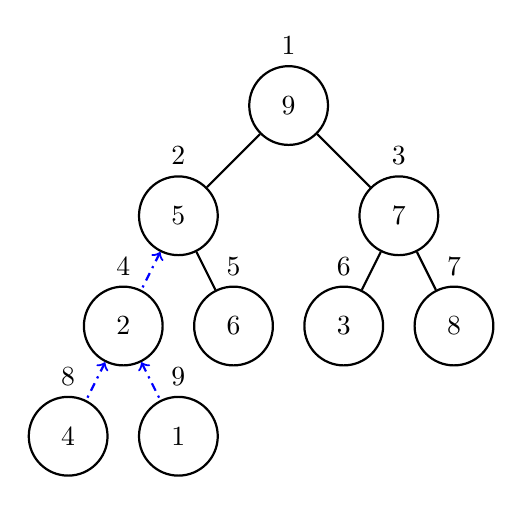
\begin{tikzpicture}[thick, scale=0.7]
        \node[label={1},circle,draw,minimum size=1cm]
        (1) at (0,0) {$9$};
        \node[label={2},circle,draw,minimum size=1cm]
        (2) at (-2,-2) {$5$};
        \node[label={3},circle,draw,minimum size=1cm]
        (3) at (2,-2) {$7$};
        \node[label={4},circle,draw,minimum size=1cm]
        (4) at (-3,-4) {$2$};
        \node[label={5},circle,draw,minimum size=1cm]
        (5) at (-1,-4) {$6$};
        \node[label={6},circle,draw,minimum size=1cm]
        (6) at (1,-4) {$3$};
        \node[label={7},circle,draw,minimum size=1cm]
        (7) at (3,-4) {$8$};
        \node[label={8},circle,draw,minimum size=1cm]
        (8) at (-4,-6) {$4$};
        \node[label={9},circle,draw,minimum size=1cm]
        (9) at (-2,-6) {$1$};

        \tikzstyle{cert}=[<-, dashdotted, blue, thick]
        \draw[thick] (1) -- (2);
        \draw[thick] (1) -- (3);
        \draw[cert] (2) -- (4);
        \draw[thick] (2) -- (5);
        \draw[thick] (3) -- (6);
        \draw[thick] (3) -- (7);
        \draw[cert] (4) -- (8);
        \draw[cert] (4) -- (9);
    \end{tikzpicture}
    \caption[Exemplo certificados do heap cinético após operação \textsc{change}]{Após a mudança de
    velocidade do elemento 2, que se encontra em \heap[$4$], os certificados
    \cert[$4$], \cert[$8$] e \cert[$9$] foram atualizados.}
    \label{fig:predeventheap}
\end{figure}

Na implementação da operação \textsc{event}, no Algoritmo~\ref{alg:abb:evento}, utilizaremos a rotina
$\textsc{update}(e)$, no Algoritmo~\ref{alg:abb:update}, que calcula o novo prazo de validade $t$
do certificado do elemento $e$, e chama a rotina~$\textsc{updatePQ}(Q, e, t)$.
A função $\textsc{swap}(e, e')$ troca a posição de $e$ e $e'$ na árvore binária balanceada
de busca e na lista ligada e a função \Call{expire}{$e,e'$} calcula
a validade do certificado entre os elementos $e$ e $e'$; se $e'$ é
\textsc{null}, retorna $+\infty$.

A função \textsc{advance} é levemente ajustada, uma vez que os prazos dos certificados não estão
mais em um vetor.

\begin{algorithm}[H]
    \caption[Algoritmo \textsc{advance}]{Função \textsc{advance}.} \label{alg:lista-ordenada:advance}
\begin{algorithmic}[1]
    \Function{advance}{$t$}
        \If{$t < $ \now}
            \State \Return
        \EndIf
        \State $i \leftarrow \Call{minPQ}{$Q$}$
        \While{$t \geq$ \cert[$i$]}
            \State \now $~\leftarrow$ \cert[i]
            \State $\Call{event}$
            \State $i \leftarrow \Call{minPQ}{$Q$}$
        \EndWhile
        \State \now $~\leftarrow$ $t$
    \EndFunction
\end{algorithmic}
\end{algorithm}

\begin{algorithm}
    \caption{Função \textsc{update}.} \label{lista:update}
\begin{algorithmic}[1]
    \Function{update}{$i$}
        \If{$1 \leq i < n$}
            \State $t \leftarrow $ \Call{expire}{$i,i+1$}
            \State \Call{updatePQ}{$Q,i,t$}
        \EndIf
    \EndFunction
\end{algorithmic}
\end{algorithm}

\begin{algorithm}
    \caption{Função \textsc{event}.} \label{torneioi:evento}
    \begin{algorithmic}[1]
        \Function{event}{\nnull}
            \State $e \leftarrow  $ \Call{minPQ}{$Q$}
            \While{$e.\cert$ = \now}
                \State $j \leftarrow e.\lastmatch$
                \State $k \leftarrow 2\cdot \floor{\frac{j}{2}}
                + ((j + 1)\mod2)$ \Comment{adversário}
                \While{$j > 1$ \AND \Call{compare}{$j, k$}}
                    \State \torneio[$\floor{\frac{j}{2}}$]
                    $\leftarrow~$\torneio[$j$]
                    \State $\torneio[k].\lastmatch$ $\leftarrow k$
                    \State \Call{update}{$\torneio[k]$}
                    \State $j \leftarrow \floor{\frac{j}{2}}$
                    \State $k \leftarrow 2\cdot \floor{\frac{j}{2}}
                    + ((j + 1)\mod2)$ \Comment{adversário}
                \EndWhile
                \State $\torneio[j].\lastmatch \leftarrow j$
                \State \Call{update}{$\torneio[j]$}
                \State $e \leftarrow  $ \Call{minPQ}{$Q$}
            \EndWhile
        % \LineComment{swapHeap$(i, \floor{\frac{i}{2}})$ troca \heap[$i$] por \heap$\left[\floor{\frac{i}{2}}\right]$}
        \EndFunction
        \LineComment{\Call{compare}{$i, j$} retorna se o valor
        de $i$ é maior que o valor de $j$.}
    \end{algorithmic}
\end{algorithm}

A operação \textsc{query\_kth}$(i)$ consiste em devolver o $i$-ésimo
maior elemento da lista ligada, ou seja, o $i$-ésimo da direita para
a esquerda, pois a árvore está em ordem crescente da esquerda para a
direita.
Para tal, percorreremos a árvore binária balanceada de busca utilizando o atributo $\children$
para, a cada iteração, decidir em qual subárvore o $i$-ésimo está, ajustando $i$ quando
necessário.
O Algoritmo~\ref{alg:abb:query} implementa esta operação e a Figura~\ref{fig:abb:queryexecution}
simula a execução em um exemplo.
A rotina auxiliar \textsc{rsize}$(r)$ devolve o valor de $r.\dir.\textit{size}$ caso $r.\dir$ seja
não nulo, caso contrário devolve $0$.

\begin{figure}[H]
    \centering
    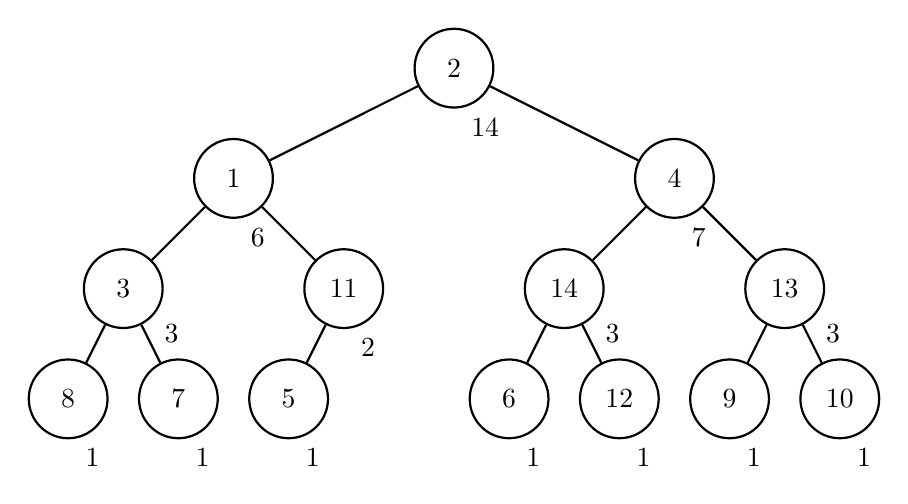
\begin{tikzpicture}[thick,scale=0.7]
        \node[label=280:{14},circle,draw,minimum size=1cm]
        (1) at (0,0) {$2$};
        \node[label=280:{6},circle,draw,minimum size=1cm]
        (2) at (-4,-2) {$1$};
        \node[label=280:{7},circle,draw,minimum size=1cm]
        (3) at (4,-2) {$4$};
        \node[label=320:{3},circle,draw,minimum size=1cm]
        (4) at (-6,-4) {$3$};
        \node[label=280:{2},circle,draw,minimum size=1cm]
        (5) at (-2,-4) {$11$};
        \node[label=320:{3},circle,draw,minimum size=1cm]
        (6) at (2,-4) {$14$};
        \node[label=320:{3},circle,draw,minimum size=1cm]
        (7) at (6,-4) {$13$};
        \node[label=280:{1},circle,draw,minimum size=1cm]
        (8) at (-7,-6) {$8$};
        \node[label=280:{1},circle,draw,minimum size=1cm]
        (9) at (-5,-6) {$7$};
        \node[label=280:{1},circle,draw,minimum size=1cm]
        (10) at (-3,-6) {$5$};
        % \node[label={11},circle,draw,minimum size=1cm] (11) at (-1,-6) {$3$};
        \node[label=280:{1},circle,draw,minimum size=1cm]
        (12) at (1,-6) {$6$};
        \node[label=280:{1},circle,draw,minimum size=1cm]
        (13) at (3,-6) {$12$};
        \node[label=280:{1},circle,draw,minimum size=1cm]
        (14) at (5,-6) {$9$};
        \node[label=280:{1},circle,draw,minimum size=1cm]
        (15) at (7,-6) {$10$};

        \draw[thick] (1) -- (2);
        \draw[thick] (2) -- (4);
        \draw[thick] (4) -- (8);
        \draw[thick] (4) -- (9);
        \draw[thick] (2) -- (5);
        \draw[thick] (5) -- (10);
        % \draw[thick] (5) -- (11);
        \draw[thick] (1) -- (3);
        \draw[thick] (3) -- (6);
        \draw[thick] (3) -- (7);
        \draw[thick] (6) -- (12);
        \draw[thick] (6) -- (13);
        \draw[thick] (7) -- (14);
        \draw[thick] (7) -- (15);
    \end{tikzpicture}
    \caption[Exemplo de árvore binária de busca com campo \children]{Exemplo de ABB com campo \children.}
    \label{fig:abb:query}
\end{figure}

\begin{figure}[H]
    \centering
    \begin{tikzpicture}[thick,scale=0.7]
        \tikzstyle{triangle} = [regular polygon, regular polygon sides=3]
        \node[
        label=280:{14},
        label=80:{$i = 7 \leq 7$},
        very thick,
        circle,
        draw,
        minimum size=1cm]
        (1) at (0,0) {$2$};
        \node[label=280:{6},triangle,draw,minimum size=1cm]
        (2) at (-4,-2) {};

        \node[label=280:{7},
        label=80:{$i = 7 > 3$},
        very thick,
        circle,draw,minimum size=1cm]
        (3) at (4,-2) {$4$};
        % \node[label=320:{3},circle,draw,minimum size=1cm]
        %     (4) at (-6,-4) {$3$};
        % \node[label=280:{2},circle,draw,minimum size=1cm]
        %     (5) at (-2,-4) {$11$};
        \node[label=320:{3},
        label=120:{$i = 3 > 1$},
        very thick,
        circle,draw,minimum size=1cm]
        (6) at (2,-4) {$14$};

        \node[label=320:{3},triangle,draw,minimum size=1cm]
        (7) at (6,-4) {};
        % \node[label=280:{1},circle,draw,minimum size=1cm]
        %     (8) at (-7,-6) {$8$};
        % \node[label=280:{1},circle,draw,minimum size=1cm]
        %     (9) at (-5,-6) {$7$};
        % \node[label=280:{1},circle,draw,minimum size=1cm]
        %     (10) at (-3,-6) {$5$};
        % \node[label={11},circle,draw,minimum size=1cm] (11) at (-1,-6) {$3$};
        \node[label=280:{1},
        label=120:{$i = 1 = 0 + 1$},
        very thick,
        circle,draw,minimum size=1cm]
        (12) at (1,-6) {$6$};

        \node[label=280:{1},triangle,draw,minimum size=1cm]
        (13) at (3,-6) {};
        % \node[label=280:{1},circle,draw,minimum size=1cm]
        %     (14) at (5,-6) {$9$};
        % \node[label=280:{1},circle,draw,minimum size=1cm]
        %     (15) at (7,-6) {$10$};

        \draw[thick] (1) -- (2);
        % \draw[thick] (2) -- (4);
        % \draw[thick] (4) -- (8);
        % \draw[thick] (4) -- (9);
        % \draw[thick] (2) -- (5);
        % \draw[thick] (5) -- (10);
        % \draw[thick] (5) -- (11);
        \draw[very thick] (1) -- node[above, sloped] {$i = 7$} (3);
        \draw[very thick] (3) -- node[above, sloped] {$i = 3$} (6);
        \draw[thick] (3) -- (7);
        \draw[very thick] (6) -- (12);% node[above, sloped] {$i = 1$} (12);
        \draw[thick] (6) -- (13);
        % \draw[thick] (7) -- (14);
        % \draw[thick] (7) -- (15);
    \end{tikzpicture}
    \caption[Exemplo de busca pelo $i$-ésimo]{Exemplo de busca pelo
    $7^\circ$ elemento da direita para a esquerda na árvore da
    Figura \ref{fig:abb:query}.}
    \label{fig:abb:queryexecution}
\end{figure}

\begin{algorithm}
    \caption{Função \textsc{query\_kth}.} \label{lista:query}
\begin{algorithmic}[1]
    \Function{query\_kth}{$i$}
        \If{$1 \leq i \leq n$}
            \State \Return \sorted[$i$]
        \EndIf
        \State \Return $-1$
    \EndFunction
\end{algorithmic}
\end{algorithm}

A operação \textsc{change}$(j, v)$, como implementada no Algoritmo~\ref{alg:abb:change}, consiste em
recuperar o elemento $e$ com identificador $j$, alterar seu atributo \initv~para $x_0 +
(\speed - v)\cdot now$, \textit{speed} para \textit{v} e
recalcular os eventuais certificados de que $j$ participa, que
seriam $e.cert$ e $e.next.cert$, se $e.next$ existe.
A Figura~\ref{fig:abb:change} ilustra um exemplo com os elementos afetados.

\begin{algorithm}
    \caption{Função \textsc{change}.} \label{torneioi:change}
    \begin{algorithmic}[1]
        \Function{change}{$j, v$}
            \State $e \leftarrow$ \Call{getObject}{$j$}
            \State $e.x_0 \leftarrow e.x_0+~(e.\speed -~v)~\cdot~\now$;
            \State $e.\speed \leftarrow v$
            \State $i \leftarrow e.\lastmatch$
            \State \Call{update}{$e$}
            \While{$i < n$}
                \If{$\torneio[i] = \torneio[2i]$}
                    \State $i \leftarrow 2i$
                \Else
                    \State $i \leftarrow 2i + 1$
                \EndIf
                \State $k \leftarrow 2\cdot \floor{\frac{i}{2}}
                + ((i + 1)\mod2)$ \Comment{adversário}
                \State \Call{update}{$\torneio[k]$}
            \EndWhile
        \EndFunction
    \end{algorithmic}
\end{algorithm}

\begin{algorithm}
    \caption{Função \textsc{change}.} \label{torneioi:change}
    \begin{algorithmic}[1]
        \Function{change}{$j, v$}
            \State $e \leftarrow$ \Call{getObject}{$j$}
            \State $e.x_0 \leftarrow e.x_0+~(e.\speed -~v)~\cdot~\now$;
            \State $e.\speed \leftarrow v$
            \State $i \leftarrow e.\lastmatch$
            \State \Call{update}{$e$}
            \While{$i < n$}
                \If{$\torneio[i] = \torneio[2i]$}
                    \State $i \leftarrow 2i$
                \Else
                    \State $i \leftarrow 2i + 1$
                \EndIf
                \State $k \leftarrow 2\cdot \floor{\frac{i}{2}}
                + ((i + 1)\mod2)$ \Comment{adversário}
                \State \Call{update}{$\torneio[k]$}
            \EndWhile
        \EndFunction
    \end{algorithmic}
\end{algorithm}

A operação \textsc{insert}$(v, x_t)$, como ilustrado na Figura~\ref{fig:abb:insert}, consiste em
criar um novo elemento, inicializando seus atributos com os devidos valores, inseri-lo na
árvore binária balanceada de busca e na estrutura que usamos para
recuperá-lo depois, calcular o seu certificado e inseri-lo na fila
com prioridades e, por fim, atualizar o certificado de seu sucessor,
caso exista.
Uma importante observação é que se \now~$\neq 0$, então $x_t \neq$~\initv.
Para calcular \initv, podemos utilizar a relação
${x_t = now\cdot \speed + x_0}$, que implica que ${x_0 = x_t -
\speed\cdot now}$.
O Algoritmo~\ref{alg:abb:insert} implementa esta operação.

\begin{figure}[H]
    \centering
    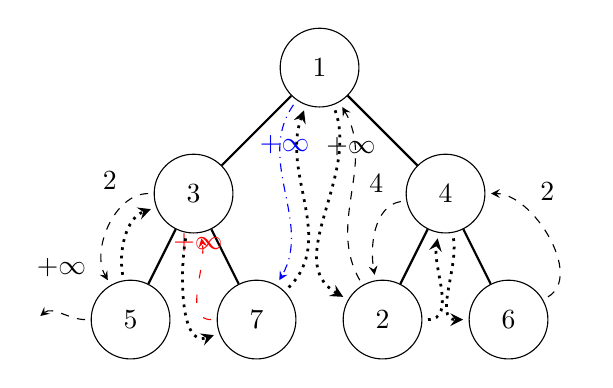
\begin{tikzpicture}[baseline=-2cm,scale=0.8]
        \node[circle,draw,minimum size=1cm] (1) at (0,0)  {$1$};
        \node[circle,draw,minimum size=1cm] (2) at (-2,-2){$3$};
        \node[circle,draw,minimum size=1cm] (3) at (2,-2) {$4$};
        \node[circle,draw,minimum size=1cm] (4) at (-3,-4){$5$};
        \node[circle,draw,minimum size=1cm] (5) at (1,-4) {$2$};
        \node[circle,draw,minimum size=1cm] (6) at (3,-4) {$6$};
        \node[circle,draw,minimum size=1cm] (7) at (-1,-4){$7$};
        % \node[label={7},circle,draw,minimum size=1cm] (7) at (3,-4) {$8$};
        % \node[label={9},circle,draw,minimum size=1cm] (9) at (-2,-6) {$1$};
        \tikzstyle{filho}=[thick]
        \tikzstyle{pred}=[->, shorten >= 2pt, shorten <= 2pt,
        dashed, >=stealth]
        \tikzstyle{sucessor}=[->, shorten >= 2pt, shorten <= 2pt,
        dotted, >=stealth, line width=0.35mm]
        % \tikzstyle{p4}=[->, shorten >= 2pt, shorten <= 2pt, dotted, >=stealth]
        \draw[filho] (1) -- (2);
        \draw[filho] (1) -- (3);
        \draw[filho] (2) -- (4);
        \draw[filho] (2) -- (7);
        \draw[filho] (3) -- (5);
        \draw[filho] (3) -- (6);
        \draw[pred] (6) edge[out=30,in=0]
        node[above=10pt] {$2$} (3);
        \draw[sucessor] (3) edge[out=280,in=180] (6);
        \draw[pred] (3) edge[out=190,in=100]
        node[above=10pt] {$4$} (5);
        \draw[sucessor] (5) edge[out=0,in=260] (3);
        \draw[pred] (5) edge[out=120,in=300]
        node[above=10pt] {$+\infty$} (1);
        \draw[sucessor] (1) edge[out=290,in=150] (5);
        \draw[pred, loosely dashed, red] (7) edge[out=180,in=280]
        node[red, above=10pt] {$+\infty$} (2);
        \draw[sucessor] (2) edge[out=260,in=200] (7);
        \draw[pred, blue, dashdotted] (1) edge[out=235,in=60]
        node[blue, above=10pt] {$+\infty$} (7);
        \draw[sucessor] (7) edge[out=45,in=250] (1);
        \draw[pred] (2) edge[out=180,in=120]
        node[above=10pt] {$2$} (4);
        \draw[sucessor] (4) edge[out=100,in=200] (2);
        \draw[pred] (4) edge[out=180,in=40]
        node[above=10pt] {$+\infty$} (-4.5, -4);
    \end{tikzpicture}
    \begin{tabular}{|c|c|c|c|c|}
        \hline
        &       &       & $\now = 1$                  \\
        $i$ & $x_0$ & $v$   & $\cert[i]$                  \\
        \hline
        $1$ & $6$   & $2$   & \textcolor{blue}{$+\infty$} \\

        $2$ & $3$   & $5$   & $+\infty$                   \\

        $3$ & $2$   & $1$   & $2$                         \\

        $4$ & $7$   & $4$   & $4$                         \\

        $5$ & $-2$  & $3$   & $+\infty$                   \\

        $6$ & $14$  & $0.5$ & $2$                         \\

        $7$ & $3$   & $1$   & \textcolor{red}{$+\infty$}  \\
        \hline
    \end{tabular}
    \caption[ABB após chamar \textsc{insert}]{Após chamar
        {\normalfont \textsc{insert}$(1, 4)$}, no instante $1$, o elemento $7$ foi
    inserido na árvore.
    O certificado do elemento $7$ foi criado e o
    certificado do seu sucessor, o elemento $1$, atualizado.}
    \label{fig:abb:insert}
\end{figure}

\begin{figure}[H]
    \centering
    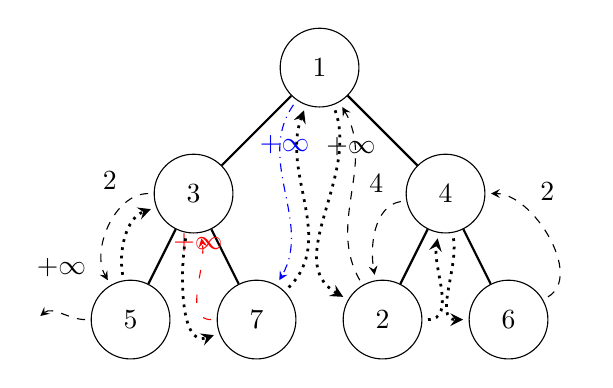
\begin{tikzpicture}[baseline=-2cm,scale=0.8]
        \node[circle,draw,minimum size=1cm] (1) at (0,0)  {$1$};
        \node[circle,draw,minimum size=1cm] (2) at (-2,-2){$3$};
        \node[circle,draw,minimum size=1cm] (3) at (2,-2) {$4$};
        \node[circle,draw,minimum size=1cm] (4) at (-3,-4){$5$};
        \node[circle,draw,minimum size=1cm] (5) at (1,-4) {$2$};
        \node[circle,draw,minimum size=1cm] (6) at (3,-4) {$6$};
        \node[circle,draw,minimum size=1cm] (7) at (-1,-4){$7$};
        % \node[label={7},circle,draw,minimum size=1cm] (7) at (3,-4) {$8$};
        % \node[label={9},circle,draw,minimum size=1cm] (9) at (-2,-6) {$1$};
        \tikzstyle{filho}=[thick]
        \tikzstyle{pred}=[->, shorten >= 2pt, shorten <= 2pt,
        dashed, >=stealth]
        \tikzstyle{sucessor}=[->, shorten >= 2pt, shorten <= 2pt,
        dotted, >=stealth, line width=0.35mm]
        % \tikzstyle{p4}=[->, shorten >= 2pt, shorten <= 2pt, dotted, >=stealth]
        \draw[filho] (1) -- (2);
        \draw[filho] (1) -- (3);
        \draw[filho] (2) -- (4);
        \draw[filho] (2) -- (7);
        \draw[filho] (3) -- (5);
        \draw[filho] (3) -- (6);
        \draw[pred] (6) edge[out=30,in=0]
        node[above=10pt] {$2$} (3);
        \draw[sucessor] (3) edge[out=280,in=180] (6);
        \draw[pred] (3) edge[out=190,in=100]
        node[above=10pt] {$4$} (5);
        \draw[sucessor] (5) edge[out=0,in=260] (3);
        \draw[pred] (5) edge[out=120,in=300]
        node[above=10pt] {$+\infty$} (1);
        \draw[sucessor] (1) edge[out=290,in=150] (5);
        \draw[pred, loosely dashed, red] (7) edge[out=180,in=280]
        node[red, above=10pt] {$+\infty$} (2);
        \draw[sucessor] (2) edge[out=260,in=200] (7);
        \draw[pred, blue, dashdotted] (1) edge[out=235,in=60]
        node[blue, above=10pt] {$+\infty$} (7);
        \draw[sucessor] (7) edge[out=45,in=250] (1);
        \draw[pred] (2) edge[out=180,in=120]
        node[above=10pt] {$2$} (4);
        \draw[sucessor] (4) edge[out=100,in=200] (2);
        \draw[pred] (4) edge[out=180,in=40]
        node[above=10pt] {$+\infty$} (-4.5, -4);
    \end{tikzpicture}
    \begin{tabular}{|c|c|c|c|c|}
        \hline
        &       &       & $\now = 1$                  \\
        $i$ & $x_0$ & $v$   & $\cert[i]$                  \\
        \hline
        $1$ & $6$   & $2$   & \textcolor{blue}{$+\infty$} \\

        $2$ & $3$   & $5$   & $+\infty$                   \\

        $3$ & $2$   & $1$   & $2$                         \\

        $4$ & $7$   & $4$   & $4$                         \\

        $5$ & $-2$  & $3$   & $+\infty$                   \\

        $6$ & $14$  & $0.5$ & $2$                         \\

        $7$ & $3$   & $1$   & \textcolor{red}{$+\infty$}  \\
        \hline
    \end{tabular}
    \caption[ABB após chamar \textsc{insert}]{Após chamar
        {\normalfont \textsc{insert}$(1, 4)$}, no instante $1$, o elemento $7$ foi
    inserido na árvore.
    O certificado do elemento $7$ foi criado e o
    certificado do seu sucessor, o elemento $1$, atualizado.}
    \label{fig:abb:insert}
\end{figure}

A operação \textsc{delete}$(i)$ consiste em recuperar o elemento
$i$, removê-lo da árvore binária balanceada de busca e da estrutura
que usamos para recuperá-lo, e depois removê-lo da fila com
prioridades.
Após isso, basta atualizar o certificado de seu sucessor, caso exista.
Essa operação é ilustrada na Figura~\ref{fig:abb:delete} e implementada no
Algoritmo~\ref{alg:abb:delete}.

\begin{figure}[htb]
    \centering
    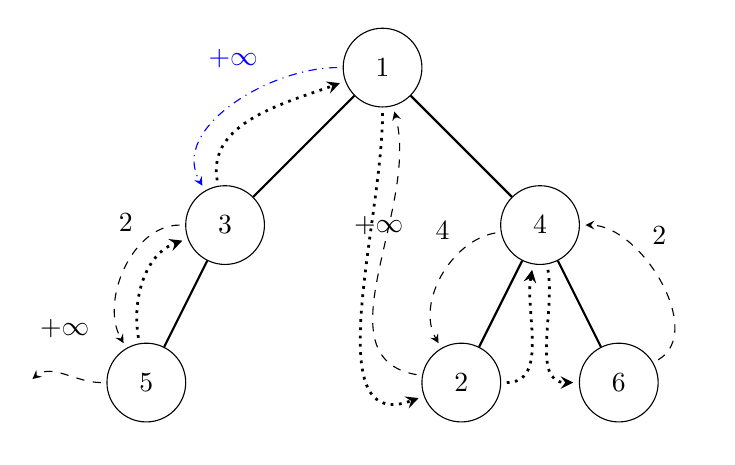
\begin{tikzpicture}[baseline=-2.25cm]
        \node[circle,draw,minimum size=1cm] (1) at (0,0)  {$1$};
        \node[circle,draw,minimum size=1cm] (2) at (-2,-2){$3$};
        \node[circle,draw,minimum size=1cm] (3) at (2,-2) {$4$};
        \node[circle,draw,minimum size=1cm] (4) at (-3,-4){$5$};
        \node[circle,draw,minimum size=1cm] (5) at (1,-4) {$2$};
        \node[circle,draw,minimum size=1cm] (6) at (3,-4) {$6$};
        % \node[label={7},circle,draw,minimum size=1cm] (7) at (3,-4) {$8$};
        % \node[label={8},circle,draw,minimum size=1cm] (8) at (-4,-6) {$4$};
        % \node[label={9},circle,draw,minimum size=1cm] (9) at (-2,-6) {$1$};
        \tikzstyle{filho}=[thick]
        \tikzstyle{pred}=[->, shorten >= 2pt, shorten <= 2pt,
        dashed, >=stealth]
        \tikzstyle{sucessor}=[->, shorten >= 2pt, shorten <= 2pt,
        dotted, >=stealth, line width=0.35mm]
        % \tikzstyle{p4}=[->, shorten >= 2pt, shorten <= 2pt, dotted, >=stealth]
        \draw[filho] (1) -- (2);
        \draw[filho] (1) -- (3);
        \draw[filho] (2) -- (4);
        \draw[filho] (3) -- (5);
        \draw[filho] (3) -- (6);
        \draw[pred] (6) edge[out=30,in=0]
        node[above=10pt] {$2$} (3);
        \draw[sucessor] (3) edge[out=280,in=180] (6);
        \draw[pred] (3) edge[out=190,in=120]
        node[above=10pt] {$4$} (5);
        \draw[sucessor] (5) edge[out=0,in=260] (3);
        \draw[pred] (5) edge[out=170,in=285]
        node[above=10pt] {$+\infty$} (1);
        \draw[sucessor] (1) edge[out=270,in=200] (5);
        \draw[pred, blue, dashdotted] (1) edge[out=180,in=120]
        node[blue, above=10pt] {$+\infty$} (2);
        \draw[sucessor] (2) edge[out=100,in=200] (1);
        \draw[pred] (2) edge[out=180,in=120]
        node[above=10pt] {$2$} (4);
        \draw[sucessor] (4) edge[out=100,in=200] (2);
        \draw[pred] (4) edge[out=180,in=40]
        node[above=10pt] {$+\infty$} (-4.5, -4);
    \end{tikzpicture}
    \begin{tabular}{|c|c|c|c|c|}
        \hline
        &       &       & $\now = 1.5$                \\
        $i$ & $x_0$ & $v$   & $\cert[i]$                  \\
        \hline
        $1$ & $6$   & $2$   & \textcolor{blue}{$+\infty$} \\

        $2$ & $3$   & $5$   & $+\infty$                   \\

        $3$ & $2$   & $1$   & $2$                         \\

        $4$ & $7$   & $4$   & $4$                         \\

        $5$ & $-2$  & $3$   & $+\infty$                   \\

        $6$ & $14$  & $0.5$ & $2$                         \\
        \hline
    \end{tabular}
    \caption[ABB após chamar \textsc{delete}]{Após chamar
        {\normalfont \textsc{delete}$(7)$} na árvore da Figura~\ref{fig:abb:insert}, o
    elemento $7$ foi retirado da árvore, a lista ligada foi
    ajustada, o certificado do seu sucessor, o elemento $1$, foi
    atualizado e o certificado do elemento $7$ foi destruído.}
    \label{fig:abb:delete}
\end{figure}

\begin{figure}[htb]
    \centering
    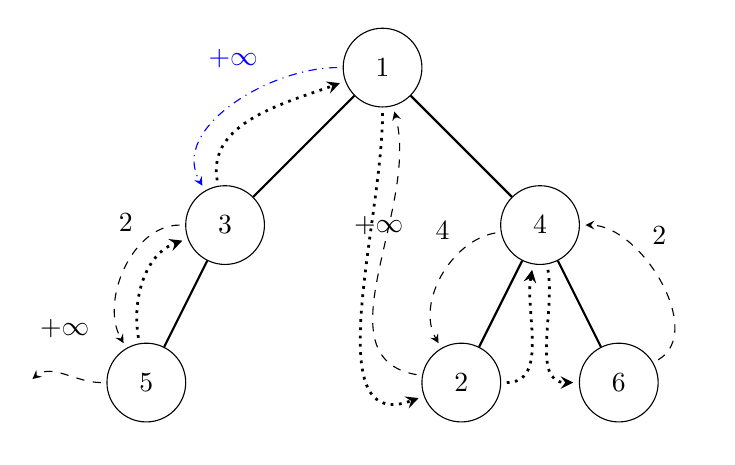
\begin{tikzpicture}[baseline=-2.25cm]
        \node[circle,draw,minimum size=1cm] (1) at (0,0)  {$1$};
        \node[circle,draw,minimum size=1cm] (2) at (-2,-2){$3$};
        \node[circle,draw,minimum size=1cm] (3) at (2,-2) {$4$};
        \node[circle,draw,minimum size=1cm] (4) at (-3,-4){$5$};
        \node[circle,draw,minimum size=1cm] (5) at (1,-4) {$2$};
        \node[circle,draw,minimum size=1cm] (6) at (3,-4) {$6$};
        % \node[label={7},circle,draw,minimum size=1cm] (7) at (3,-4) {$8$};
        % \node[label={8},circle,draw,minimum size=1cm] (8) at (-4,-6) {$4$};
        % \node[label={9},circle,draw,minimum size=1cm] (9) at (-2,-6) {$1$};
        \tikzstyle{filho}=[thick]
        \tikzstyle{pred}=[->, shorten >= 2pt, shorten <= 2pt,
        dashed, >=stealth]
        \tikzstyle{sucessor}=[->, shorten >= 2pt, shorten <= 2pt,
        dotted, >=stealth, line width=0.35mm]
        % \tikzstyle{p4}=[->, shorten >= 2pt, shorten <= 2pt, dotted, >=stealth]
        \draw[filho] (1) -- (2);
        \draw[filho] (1) -- (3);
        \draw[filho] (2) -- (4);
        \draw[filho] (3) -- (5);
        \draw[filho] (3) -- (6);
        \draw[pred] (6) edge[out=30,in=0]
        node[above=10pt] {$2$} (3);
        \draw[sucessor] (3) edge[out=280,in=180] (6);
        \draw[pred] (3) edge[out=190,in=120]
        node[above=10pt] {$4$} (5);
        \draw[sucessor] (5) edge[out=0,in=260] (3);
        \draw[pred] (5) edge[out=170,in=285]
        node[above=10pt] {$+\infty$} (1);
        \draw[sucessor] (1) edge[out=270,in=200] (5);
        \draw[pred, blue, dashdotted] (1) edge[out=180,in=120]
        node[blue, above=10pt] {$+\infty$} (2);
        \draw[sucessor] (2) edge[out=100,in=200] (1);
        \draw[pred] (2) edge[out=180,in=120]
        node[above=10pt] {$2$} (4);
        \draw[sucessor] (4) edge[out=100,in=200] (2);
        \draw[pred] (4) edge[out=180,in=40]
        node[above=10pt] {$+\infty$} (-4.5, -4);
    \end{tikzpicture}
    \begin{tabular}{|c|c|c|c|c|}
        \hline
        &       &       & $\now = 1.5$                \\
        $i$ & $x_0$ & $v$   & $\cert[i]$                  \\
        \hline
        $1$ & $6$   & $2$   & \textcolor{blue}{$+\infty$} \\

        $2$ & $3$   & $5$   & $+\infty$                   \\

        $3$ & $2$   & $1$   & $2$                         \\

        $4$ & $7$   & $4$   & $4$                         \\

        $5$ & $-2$  & $3$   & $+\infty$                   \\

        $6$ & $14$  & $0.5$ & $2$                         \\
        \hline
    \end{tabular}
    \caption[ABB após chamar \textsc{delete}]{Após chamar
        {\normalfont \textsc{delete}$(7)$} na árvore da Figura~\ref{fig:abb:insert}, o
    elemento $7$ foi retirado da árvore, a lista ligada foi
    ajustada, o certificado do seu sucessor, o elemento $1$, foi
    atualizado e o certificado do elemento $7$ foi destruído.}
    \label{fig:abb:delete}
\end{figure}

\FloatBarrier

\subsection{Análise de desempenho}\label{subsec:analise-de-desempenho-abb}

A árvore binária balanceada de busca é uma estrutura \textit{responsiva}, pois o
custo de processar um certificado é $O(\lg{n})$, onde $n$ é o número de elementos sendo mantidos,
que é o custo da rotina \textsc{event}, que atualiza a posição dos elementos na árvore em $O(1)$ e
realiza alterações na fila de certificados em tempo $O(\lg{n})$.

Assim como a lista ordenada cinética, a árvore binária balanceada de busca é uma
estrutura \textit{eficiente}, \textit{compacta} e \textit{local}, pelas mesmas
justificativas apresentadas na Seção~\ref{sec:lista}.

Apesar do mesmo bom desempenho que a lista ordenada cinética nestas operações, a árvore de busca
binária balanceada realiza a operação \textsc{query-kth} em $O(\lg{n})$, que é um
desempenho assintótico pior em relação à lista ordenada cinética, que realiza a
mesma operação em $O(1)$.

O desempenho pior na operação \textsc{query-kth} é justificado pelo ganho de
desempenho nas operações \textsc{insert} e \textsc{delete}, que também são
realizadas em tempo $O(\lg{n})$, enquanto que na lista ordenada cinética o tempo
gasto é seria$O(n)$, pois precisaríamos mover $O(n)$ objetos para posicionar o novo
elemento na posição correta ou para reorganizar o vetor de forma a ocupar a
posição que ficou vazia após a remoção de um elemento.
